\documentclass[conference, 11pt]{IEEEtran}
\IEEEoverridecommandlockouts
% The preceding line is only needed to identify funding in the first footnote. If that is unneeded, please comment it out.
\usepackage{cite}
\usepackage{amsmath,amssymb,amsfonts}
\usepackage{algorithmic}
\usepackage{graphicx}
\usepackage{textcomp}
\usepackage{xcolor}
\def\BibTeX{{\rm B\kern-.05em{\sc i\kern-.025em b}\kern-.08em
    T\kern-.1667em\lower.7ex\hbox{E}\kern-.125emX}}
\usepackage{hyperref}
%Removing indentation.
\newlength\tindent
\setlength{\tindent}{\parindent}
\setlength{\parindent}{0pt}
\renewcommand{\indent}{\hspace*{\tindent}}
\usepackage{float}

\begin{document}

\title{Rain Detection Measurement System Using Infrared Transceiver\\
{\footnotesize \textsuperscript{}ELEN4006}
}

\author{\IEEEauthorblockN{1\textsuperscript{st} Darren Blanckensee}
\IEEEauthorblockA{\textit{School of Electrical and Information Engineering} \\
\textit{University of the Witwatersrand}\\
Johannesburg, South Africa \\
1147279@students.wits.ac.za}
\and
\IEEEauthorblockN{2\textsuperscript{nd} Uyanda Mphunga}
\IEEEauthorblockA{\textit{School of Electrical and Information Engineering} \\
\textit{University of the Witwatersrand}\\
Johannesburg, South Africa \\
1168101@students.wits.ac.za}
}

\maketitle

\begin{abstract}
UUUUUUUUYYYYYYYAAAAAAANNNNNNNNDDDDDDDDDAAAAAAAAA
\end{abstract}

\begin{IEEEkeywords}

\end{IEEEkeywords}

\section{Introduction}
\IEEEPARstart{T}{he} purpose of this project is design and simulate a rain detection measurement system for an electric vehicle. The system is to be mounted under the rear view mirror and uses an infrared transmitter and receiver pair to determine the amount of water on the section of the windshield that is observable by the measurement system. It is a fair assumption that if the amount of water on any section of the windshield is representative of the amount of water on the whole windshield.  This measurement systems purpose is not only to display to the driver how much water is on the windshield and by extension how hard it is raining but also to be able to generate an input to the PWM system that controls the speed of the windshield wipers. The measurement system's design is based on the fundamental principles of measurement systems and the model given in Bentley \cite{BENT}. There are four main sections to this measurement system, namely the sensing stage, the signal conditioning stage, the signal processing stage and the data presentation stage. \\


The sensing stage involves the infrared transmitter and receiver pair. The signal conditioning stage includes the filter which acts as a noise removal filter as well as an anti-aliasing filter. The signal processing stage takes place within the ADC where voltages are related to different levels of rain and the corresponding outputs to the user and the windshield PWM are produced. The smartness of the system is in the ability to calibrate at will which can be used as a means of customising the speed at which the windshield wipers operate as different drivers may have different preferences as to how different levels of rain relate to to certain speeds. The value of this measurement system is that it reduces the number of distractions that occur during the driving process. Driving in the rain is dangerous and having to monitor and adjust the windshield wipers manually is an unnecessary distraction that will with the help of this measurement system be eliminated. Furthermore this report details the static and dynamic characteristics of the designed measurement system. Lastly the Strengths Weaknesses Advantages and Threats~(SWAT) of the measurement system are evaluated and the conclusion then summarises the key points from each section and analyses the successes and failures of this design. 

\section{Background}
	
	
	
\subsection{Measurement Systems}
UUUUUUUUYYYYYYYAAAAAAANNNNNNNNDDDDDDDDDAAAAAAAAA

	
\subsection{Literature Survey}
The use of infrared transceivers (transmitter receievr pairs) in rain detection is not new and has been around since 1958 \cite{SENS}. There are a number of ways to detect rain on the windshield of a car. This report focuses on the use of an infrared transceiver. In \cite{NOTE} the use of a Greenpak SLG46620V integrated circuit in conjunction with the infrared transmitter and receiver allows for great control of a number of characteristics of the measurement system. This was seen as being too complex and did not leave much to design however the transmitter and receiver circuits used in this report are loosely based on those in \cite{NOTE}. 
Furthermore in \cite{NOTE} it is suggested that a single order low pass filter be used at the output however it became clear during the design process that this was not sufficient and so a second order filter was chosen. In
\cite{PULSE} a circuit for pulse generation using a microcontroller (PIC16F876-20) is given. This will be used in the transmitter circuit. 


	
\subsection{Optics and the Use of Total Internal Reflection}
When light passes through a medium and meets a boundary, if the medium on the other side of the boundary has a lower refractive index than the medium the light is already in and the light strikes this boundary with an angle greater than the critical angle the light is totally internally reflected. When the refractive index of the medium on the other side of the boundary is greater then some of the light is refracted out of the medium and less light is therefore internally reflected. \\

This measurement system takes advantage of this physical phenomenon by shotting infrared light into the windshield at an angle higher than the critical angle calculated to be $41.08 ^{\circ}$ given that the refractive index of air is $1.0003$ and using the average refractive index of windshield glass determined in \cite{RI} to be approximately $1.522$. When there is water on the glass the refractive index on the outside boundary changes from $1.0003$ to $1.333$ which changes the critical angle from $41.08 ^{\circ}$ to $61.14 ^{\circ}$. It is therefore decided that the infrared light be shot at the windshield at an angle of $45 ^{\circ}$ such that when there is no water the light will be totally internally refracted but when water is present the some of the light will be refracted and the received amount of light will be less than what was sent indicating the presence of water. This concept is clearly illustrated in the system block diagram in the Design section below. 

	
\subsection{Real World Challenges (Noise and Its Effects)}
UUUUUUUUYYYYYYYAAAAAAANNNNNNNNDDDDDDDDDAAAAAAAAA
---------------------- NEEEEEEDS MORE -------------
\cite{NOISE}
	
\section{Design}
This section deals with the design of each of each of the stages shown in the system block diagram in figure 1 that form part of this measurement system. 

 \begin{figure}[H]
 \centering 
 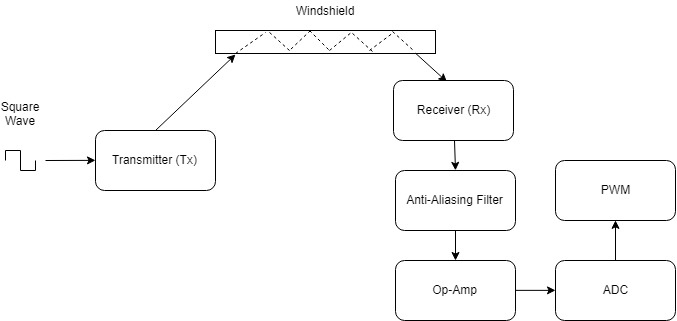
\includegraphics[width=\columnwidth]{SystemBlockDiagram}
 \centering 
  \caption {System block diagram. }
 \end{figure}
 
 Each of these blocks fall into one of the predefined stages in the Bentley model and are explained in depth in the subsections to follow.
 
 \subsection{Transmitter}
 The Infrared transmitter chosen for this system was the IR928-6C-F. It was chosen for its Peak wavelength $λp=940nm$ (chosen because it matches the receivers emitter wavelength) and its low forward voltage of $1.2V$. The transmitter circuit is setup as a typical LED driver circuit with the LED being replaced by the infrared transmitter and the voltage source is replaced by the pulse generator described in the literature review section above. This pulse generator has a period of $1ms$ and a pulse width of $10\mu s$ The Darlington NPN transistor TIP121 was also used. The circuit can be seen in the full system circuit diagram in the appendix. The need for a pulse generator is due to the operating temperature range of the transistor used. If the transistor is on 100\% of the time the power dissipated is 4W which leads to an operating temperature of $275 ^{\circ}C$ which is $125 ^{\circ}C$ above the temperature range specified in the datasheet \cite{TP121}. Therefore it was decided that the pulse generator be used to ensure a duty cycle of 1\% which leads to an operating temperature of $27 ^{\circ}C$ which falls well within the specified range. The output of the transmitter circuit is the voltage difference across the infrared transmitter that produces the infrared light that is shot into the windshield. Graphs of this output can be seen in the simulations section. 

\subsection{Receiver}
The receiver used in this system was the CNY70 reflective optical sensor. It was chosen for its emitter peak wavelength of $940 nm$ which is exactly the same as the peak wavelength of the transmitter and so the light sent by the transmitter will definitely be received by the receiver. The receiver circuit can be seen in the appendix. When light is received by the receiver current is allowed to flow through the circuit which through a resistor produces a voltage. This voltage at the output is expected to be very close to that of the output of the transmitter if there is no rain on the windshield. In the real world however, the matter is not that simple as there is a significant amount of infrared noise in the environment and this needs to be catered for by the system. Due to this when modeling the circuit a noise source was added as the supply to another transmitter circuit that would also be picked up at the receiver just as it would be in the real world. The output of the receiver is a shifted pulse depending on the amount of light received this DC component of the signal can vary between 1 and 6.5 Volts (maximum should be 5V but simulations show noise can shift the signal by as much as 1.5V). These values (1 and 5  Volts) are to be stored by the Microcontroller used in the ADC stage as the values corresponding to heavy rain and no rain respectively. Graphs of the receivers output with rain and without can be seen in the simulations section. 

\subsection{Anti-Aliasing}
In any system that is to be converted from analog to digital it is important to have an Anti-Aliasing filter so as to avoid signal distortion introduced by sampling the signal \cite{FILT}. In this system the output of the signal as shown by the simulations contains a large amount of noise which is not ideal and needs to be dealt with and the authors saw the anti-aliasing filter as an opportunity to deal with the noise while simultaneously catering for the aliasing issues that would otherwise be introduced in the sampling stage. The filter used is a second order low pass filter in Sallen-Key topology with a band pass frequency of $2000Hz$ which is twice the frequency of the pulse at the receiver. The noise is very high frequency and will therefore be eliminated. The circuit for this filter is shown as part of the full circuit diagram in the appendix. The output of the filter is a relatively straight line that resides within a certain voltage range that relates to the amount of water on the windshield. The higher the voltage the less infrared light was lost which means not a lot of water was present on the windshield. The bode plot and step response of the filter is shown in figure 2 below. 

 \begin{figure}[H]
 \centering 
 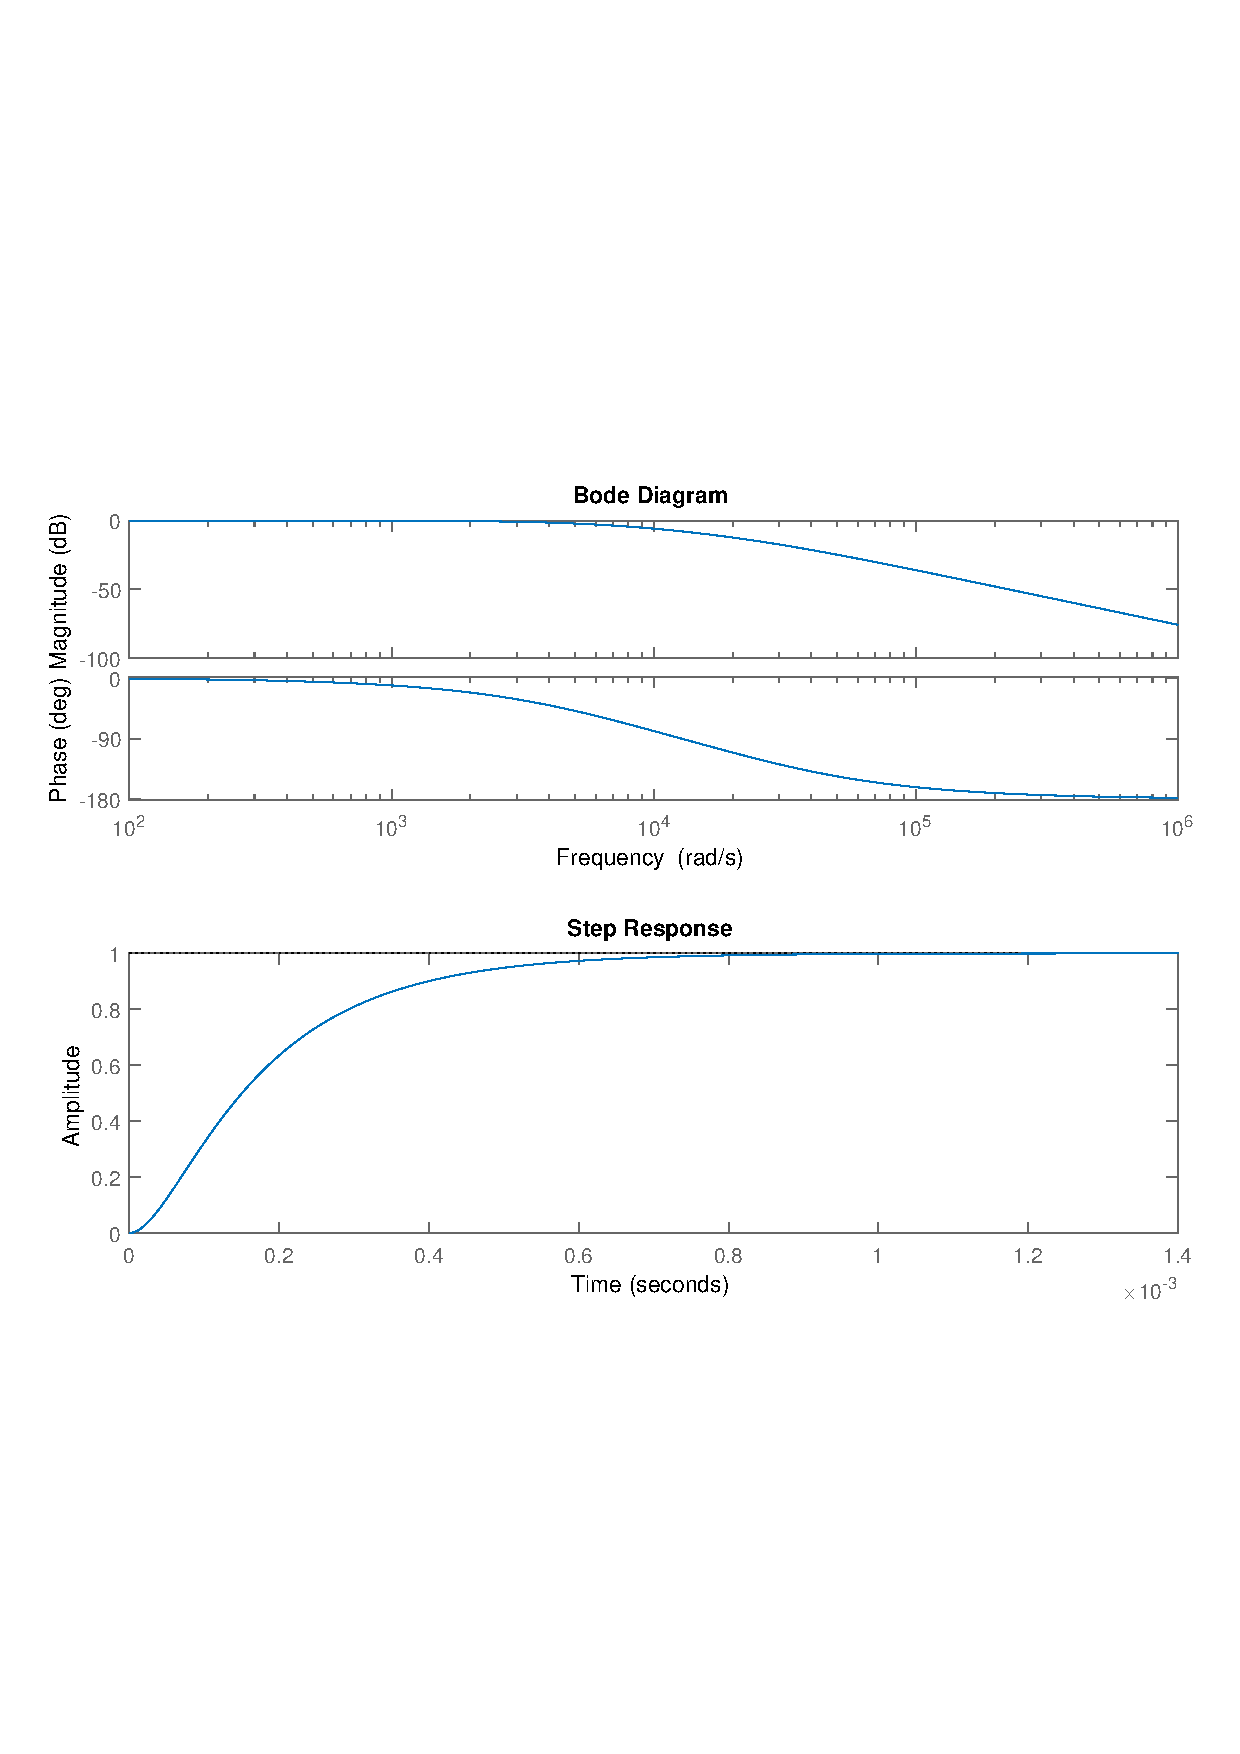
\includegraphics[width=\columnwidth]{BodeStep}
 \centering 
  \caption {Filter Bode Plot. }
 \end{figure}

As can be seen from the step response the filter settles within a time of $0.7ms$. The bandwidth of the filter is $2000Hz$ as can be seen from the bode diagram. The simulated output of the filter can be seen in the simulation section. 


\subsection*{ADC}
The analog to digital conversion will be done using a MAX1132 which has a resolution of 16 bits. It was chosen for its high signal to noise ratio of 89dB and its high resolution \cite{ADC}. The ADC will have preset voltage ranges stored that relate to certain rain levels and therefore wiper speeds. For example If the voltage is $5$ $\pm 0.3V$ or above then there is no rain. If the voltage is between 4 and 5 volts then there is a slight drizzle and the wipers should be on at their lowest speed. If the value is between 3 and 4 Volts then the wipers should be on moderately fast or on their "medium setting". If the value is between 2 and 3V then the wipers should be on fast and if the voltage is below 2V then the wipers should be at their absolute maximum speed.

\subsubsection{Smartness}
The smartness of the system is in the calibration method and what power it gives the driver over the speeds at which the automatic wipers responds to certain rain levels. With this system being able to store the range values in the memory of the ADC at any particular time the driver is able to change these values using the display button. The driver might prefer to have their wipers on at their maximum speed at a rain level that corresponds to a voltage of 3V. This is a personal preference and may be different for every individual driver. The measurement system when the button to set the new maximum speed rain level (the rain level at which the driver feels the wipers should be on at full speed) is pressed will save this value in the ADC in the voltage ranges and will recalculate all other ranges accordingly so that each speed corresponds to a certain voltage range as described above. The output of the ADC can then be used to display to the user the level of rain it is measuring at any given point in time. This will be done through four LEDs next to a picture of a cloud with rain coming out of it on the dashboard then similarly to the way in which the fuel pump image lights up when fuel is needed the rain gauge will light up along with a either one, two, three or four of the LEDs next to it. No LED being on indicates that there is no rain, four LEDs being on indicates heavy rain. The driver is then able to get a feel for what the measurement system understands to be heavy rain vs light drizzles and this knowledge can bu used to personalise the measurement system as described above so as to better suit the driver. 


\section{Simulation Results}
This section explains the measurement process from beginning to end. From the time the measurement system is first used to shoot infrared light into the windshield to the time the rain level is shown to the driver and the PWM signal is generated by the ADC. Figure 3 below shows three key signals when there is no rain present and those same signals when there is rain present. These three key signals are the output of the transmitter, the output of the receiver and the output of the anti-aliasing and anti-noise filter. 

 \begin{figure}[H]
 \centering 
 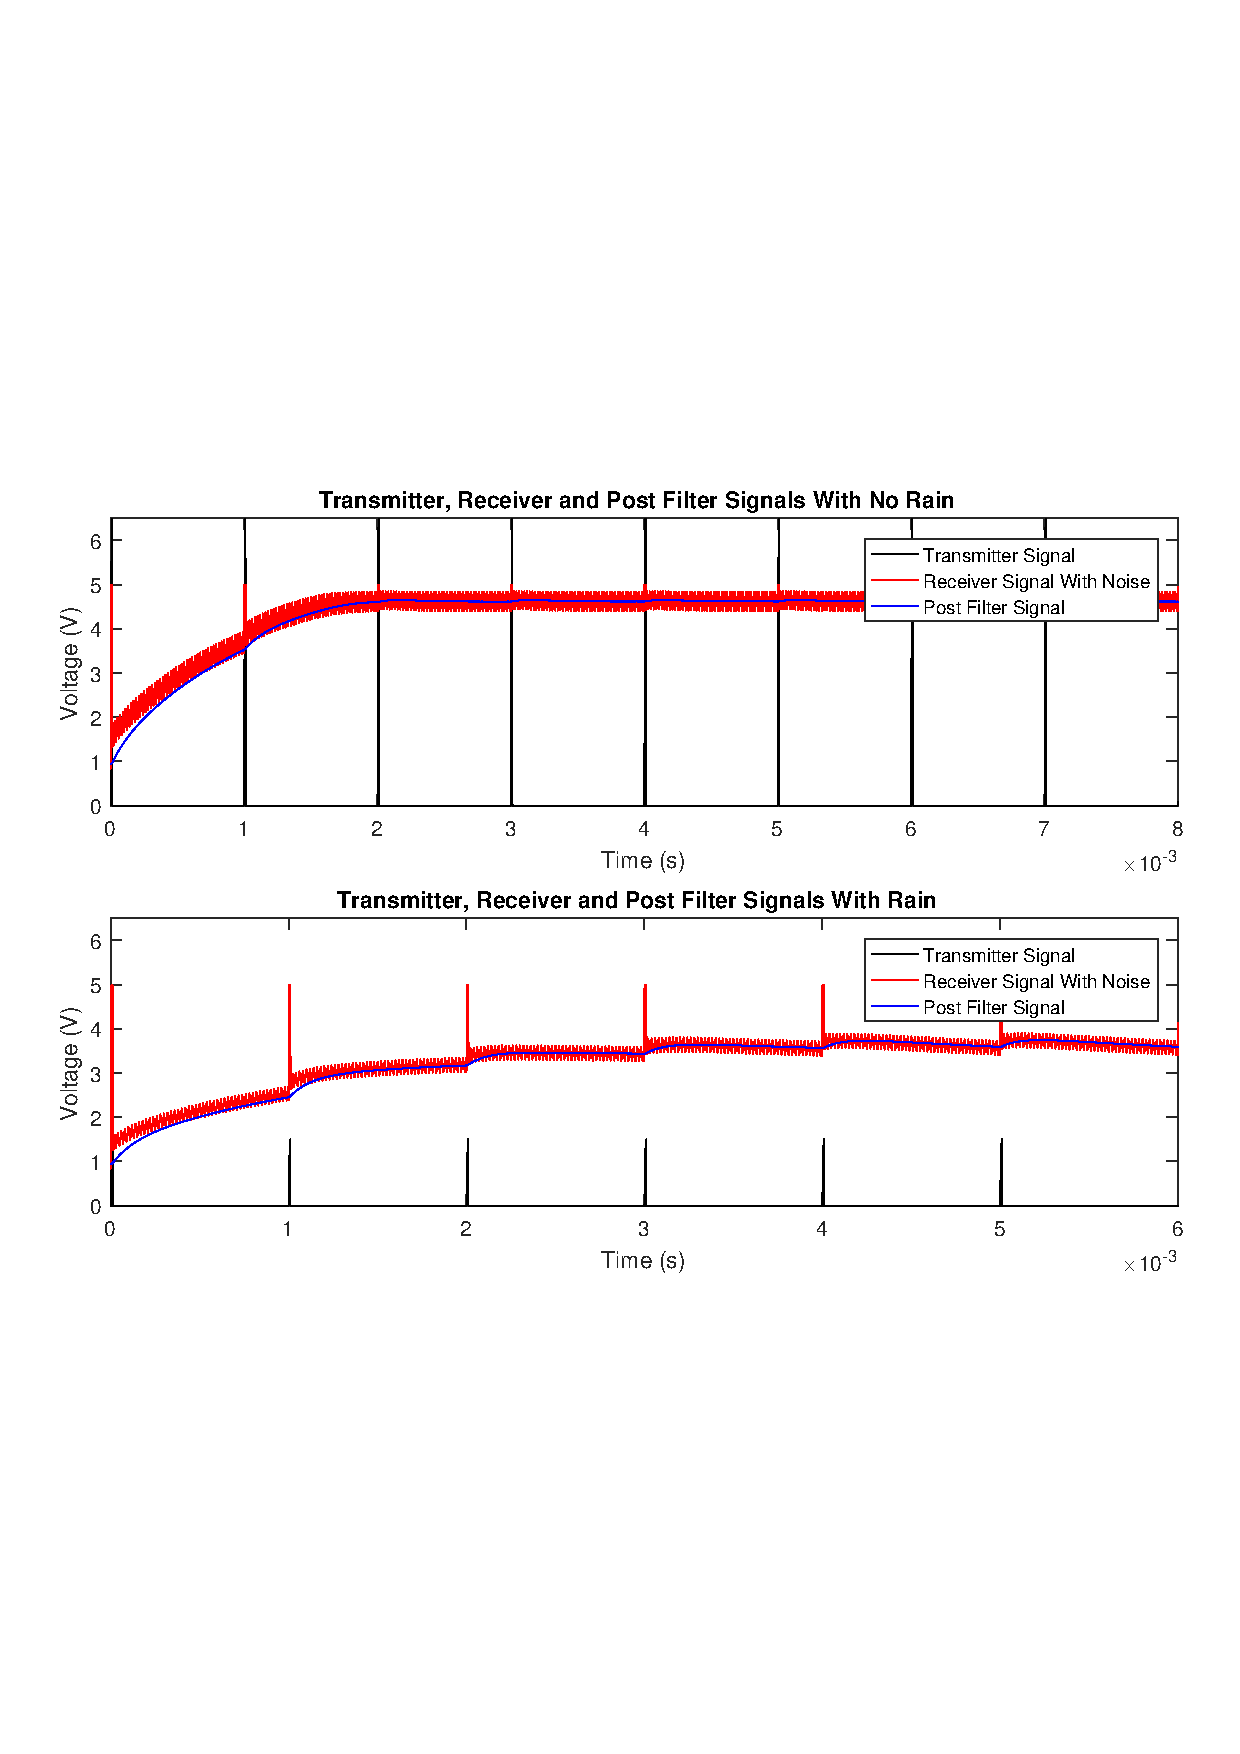
\includegraphics[width=\columnwidth]{RainVsNoRain}
 \centering 
  \caption {System Simulations. }
 \end{figure}

One important thing to note about this simulation is that it can easily be seen that the settling time of this system pre-ADC is approximately $4ms$. This is significantly slower than that of the filter however it is still more than fast enough as the intensity of the rain is not going to change drastically in $4ms$. \\

As can be seen in the graphs above the signal at the receiver is extremely noisy due to various sources of infrared light interfering with the signal that is intended to be received. The filter gets rid of this noise and results in a smooth curve that can easily be fed to the ADC and used to check within which range it falls and therefore determine how heavy it is raining if at all. As the amount of water droplets increases more and more light will leave the windshield and so less light will be received at the receiver meaning the voltage signal that is filtered will have a lower average value resulting in the blue line of the graph being shifted even lower. This would cause the ADC to identify that the amount of rain has increased and it will then send the appropriate signals to the dashboard display as well as the PWM of the wipers. 


\section{Static and Dynamic Characteristics}

\subsection{Resolution}
Given that the systems ADC has a resolution of 16 bits and the highest values it needs to read is 5V this means that the lowest change in voltage  that can happen without change in the ADC value and therefore its resolution in terms of voltage is $76.3\mu V$. Which  is more than sufficient especially when considering that there are only five speed levels including off. 

\subsection{Operating Temperature}
The operating temperature is determined by the most strict of all the components involved and is therefore between $0$ and $70^{\circ}C$. 

\subsection{Steady State Error}
Error in this context is difficult to conceptualise as the measurement system is not directly measuring the amount of water on the windshield but rather inferring from how much light is lost how intense the rain is. Therefore determining error becomes complicated. The ADCs maximum off set and gain error is 6mV which out of 5V is 0.12\%. 


\subsection{Settling Time}
The settling time as mentioned above is approximately $4ms$ which means that the system is more than capable of handling fast changing weather conditions. 

\subsection{Dynamic Error}
It can be seen in figure 3 that the dynamic error is more significant than the static error as the blue line fails to accurately match at of the noisy red line. The gretaest difference is at the beginning just after the input is applied. The error at this point is 20\%. It is important to note however that the input mirrors a situation where there is no rain whatsoever and then all of a sudden there is a constant level of rain. This however would never happen in real life and so the dynamic error can be neglected.  


\section{SWAT Analysis}
\subsection{Strengths}
The strengths of this system are:
\begin{itemize}
\item Fast response time of $4ms$.
\item Allows for personalisation through calibration (smartness).
\item Eliminates noise effectively from system.
\item Is able to operate in high temperatures (maximum of $70^{\circ}C$).
\item Parts are widely available. 
\end{itemize}

\subsection{Weaknesses}
The weaknesses of this system are:
\begin{itemize}
\item requires two micocontrollers, one for pulse generation at transmitter and one for analog to digital conversion. Would be ideal to have one for both. 
\item Is not able to operate at temperatures below $0^{\circ}C$ and is therefore limited in where it can be deployed. 
\item No logical checks have been implemented to ensure that calibrations done by the drivers are sensible. For example if driver sets their max rain level to be when there is no rain then the wipers will be on full speed constantly even when there is no rain at all. 
\item Various voltage sources of different magnitudes are needed namely 12V and 5V. would be ideal to have just one ideally the 12V as that is obtainable from the battery itself. 
\end{itemize}

\subsection{Advantages}
One advantage of this measurement system is that it allows the driver to focus more carefully on the road. This will result in many lives being saved as statistics relating to motor vehicle related deaths are high as drivers are often distracted by a number of things. Removing one of these distractions will help drivers remain safe on the roads. Another advantage is the ability to personalise the settings of the meausrement system to be able to control how much rain needs to be present for the wipers to operate at certain speeds.

\subsection{Threats}
As stated in weaknesses the lack of logical checks when personalising the operations of the system could lead to the wipers being on all the time even if there is no rain. While the user could just re-calibrate and fix the issue themselves it is not ideal and could be more of a distraction than having to control the wiper speed themselves. This can be fixed within the ADC by declaring a minimum level of rain that has to be present for the calibration of max rain level to be accepted.



\section{Conclusion}
UUUUUUUUYYYYYYYAAAAAAANNNNNNNNDDDDDDDDDAAAAAAAAA


\begin{thebibliography}{22}

	%Each item starts with a \bibitem{reference} command and the details thereafter.

\bibitem{BENT} 
John P. Bentley. \\
\textit{Principles Of Measurement Systems Fourth Edition}. \\
Pearson Education Limited 1983, 2005



\bibitem{SENS} 
Alexandru Vasile, Irina Vasile, Adrian Nistor, Luige Vladareanu, Mihaela Pantazica, Florin Caldararu, Andreea Bonea, Andrei Drumea, Ioan Plotog.\\
\textit{Rain sensor for automatic systems on vehicles}. \\
Proc. SPIE 7821, Advanced Topics in Optoelectronics, Microelectronics, and Nanotechnologies V, 78211W (4 December 2010)

\bibitem{NOTE} 
Dialog Semiconductor. \\
\textit{Application Note IR Windshield Rain Sensor AN-1219}. \\
CFR0014 2 of 23 © Dialog Semiconductor, 2018.


\bibitem{RI} 
Crystal Munger,1 M.S.F.S.; Kris M. Gates,2 B.S., M.A.T.; and Christopher Hamburg,2 B.S. \\
\textit{Determining the Refractive Index Variation within Panes of Vehicle Windshield Glass}. \\
J Forensic Sci, September 2014, Vol. 59, No. 5.



\bibitem{NOISE} 
Łukasz Ciura, Andrzej Kolek, Waldemar Gawron, Andrzej Kowalewski, Dariusz Stanaszek.\\
\textit{MEASUREMENTS OF LOW FREQUENCY NOISE OF INFRARED PHOTO- DETECTORS WITH TRANSIMPEDANCE DETECTION SYSTEM}. \\
METROLOGY AND MEASUREMENT SYSTEMS\\
2014 Polish Academy of Sciences.



\bibitem{PULSE} 
Miloslav HRUŠKOVIC, Ján HRIBIK \\
\textit{Pulse Generator Controlled by Microcontroller}. \\
1 Dept. of Radio Electronics, Slovak University of Technology, Ilkovičova 3, 812 19 Bratislava, Slovak Republic


\bibitem{TP121} 
DARLINGTON TIP120, TIP121, TIP122 (NPN); TIP125, TIP126, TIP127 (PNP)\\
\textit{Plastic Medium-Power Complementary Silicon Transistors}. \\
On Semiconductor


\bibitem{FILT} 
Stefano Bregni, Franco Setti.\\
\textit{Impact of the Anti-Aliasing Pre-Filtering on the Measurement of Maximum Time Interval Error}. \\
0-7803-4198-8/97/\$10.00 0 1997 IEEE


\bibitem{ADC} 
Maxim MAX1132/MAX1133.\\
\textit{16-Bit ADC, 200ksps, 5V Single-Supply with Referencer}. \\
9-2083; Rev 0; 8/01



\bibitem{CHAR}

\textit{STATIC \& DYNAMIC CHARACTERISTICS OF MEASUREMENT SYSTEM}
\url{http://mediatoget.blogspot.in/2012/01/static-dynamic-characteristics- of.html}

\end{thebibliography}
\end{document}
